\chapter{Resultater og analyse fra Case 3: Misbruk av NTNU sin infrastruktur til utvinning av kryptovaluta}
I dette kapittelet fremlegger vi våre resultater i alle fasene i case 3.
%%%%%%%%%%%%%%%%%%%%%%%%%%%%%%%%%%%%%%%%%%%%%%%%%%%%%%%%%%%%%%%%%%%%%
\section{Problemforståelse}
\subsection{Ytelsesmatrise}
Variablene som ble vurdert til å kunne hjelpe til å redusere utvinning av kryptovaluta hos NTNU er som følger:
\begin{description}
    \item[Adgangskontroll på HPC klynger:] Klynger av tilkoblet maskinvare som sammen utgir svært høy ytelse. Er også kjent som superdatamaskiner. Disse er godt beskyttet med streng adgangskontroll og logging av alt som blir gjort.
    \item[Adgangskontroll på kritiske servere:] Adgangskontroll til servere som har en funksjonskritisk og/eller virksomhetskritisk rolle i driften av NTNU, som for eksempel DNS og DHCP servere. 
    \item[Adgangskontroll på andre servere:] Adgangskontroll til alle servere som ikke har en kritisk rolle i NTNU, men som fortsatt kan bli misbrukt. Inkluderer servere som står åpent ut mot nettet. 
    \item[Beskyttelse mot ufrivillig utvinning på datamaskiner:] Personer får tilgang til din datamaskin gjennom nettleseren og bruker den til å utvinne kryptovaluta. 
    \item[Policy på hva som er akseptabelt som BYOD:] Definerer hva som er lov å ta med av BYOD.
    \item[IT-reglement på krypto utvinning:] IT-reglementet spesifiserer per idag bare at det å bruke universitetets ressurser til kommersiell virksomhet ikke er greit. Det kan være vanskelig for folk å ta koblingen til at strøm er en slik ressurs og at utvinning av kryptovaluta kan regnes som kommersiell virksomhet. Sånn som IT-reglementet er idag er det heller ikke noen gode sanksjonsmuligheter mot folk som utvinner kryptovaluta.
\end{description}

Under ser vi hvor de ulike ressursene, eller aktiva, er plassert i henhold til de tidligere nevnte områdene.
\begin{figure}[H]
    \centering
    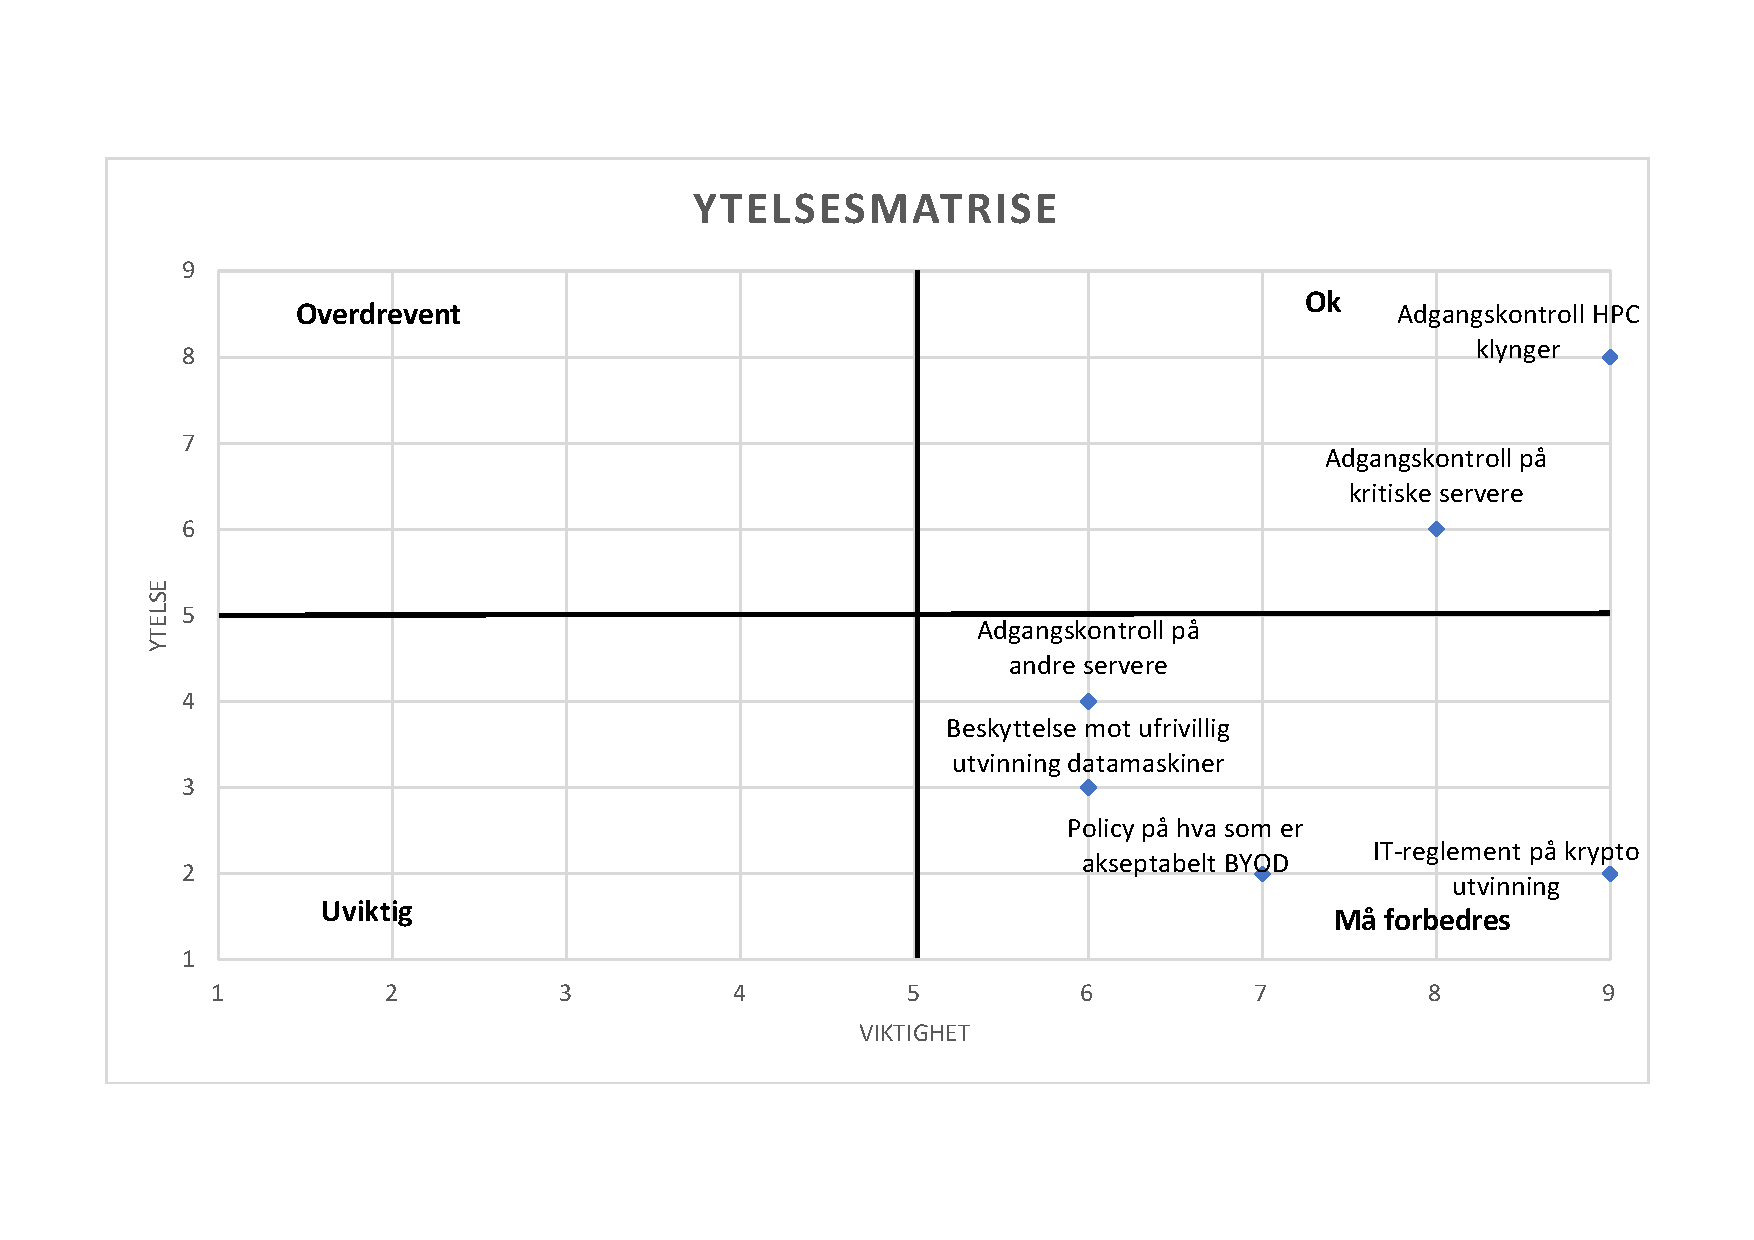
\includegraphics[scale=0.5]{case_3/bilder/ytelsesmatrise.pdf}
    \caption[Ytelsesmatrise]{Resultater fra ytelsesmatrisen}
    \label{fig:ytelsesmatrise}
\end{figure}

Det er mest kritisk å vurdere de variablene som havner under ``må forbedres''. Selv om noen havner under ``ok'', bør de fortsatt vurderes, men de vil ha lavere prioritet enn de nevnt over. Variabler som er uviktig eller overdrevent trenger man ikke vurdere nøye. Matrisen viser følgende prioriteringsgrunnlag til utbedring:

\begin{enumerate}
    \item IT-reglement på krypto utvinning
    \item Policy på hva som er akseptabelt som BYOD
    \item Beskyttelse mot ufrivillig utvinning på datamaskiner
    \item Adgangskontroll på andre servere
    \item Adgangskontroll på kritiske servere
    \item Adgangskontroll på HPC klynger
\end{enumerate}

%%%%%%%%%%%%%%%%%%%%%%%%%%%%%%%%%%%%%%%%%%%%%%%%%%%%%%%%%%%%%%%%%%%%%
\section{Idémyldring}
\subsection{Idémyldring}
Etter at idémyldringsøkten var ferdig ble det gjort en vurdering av hvilke momenter som hørte sammen eller hadde likhetstrekk.  Disse ble gruppert sammen, se figur \ref{fig:idemyldring-hvordan} og \ref{fig:idemyldring-hvorfor} under.

\begin{figure}[H]
    \centering
    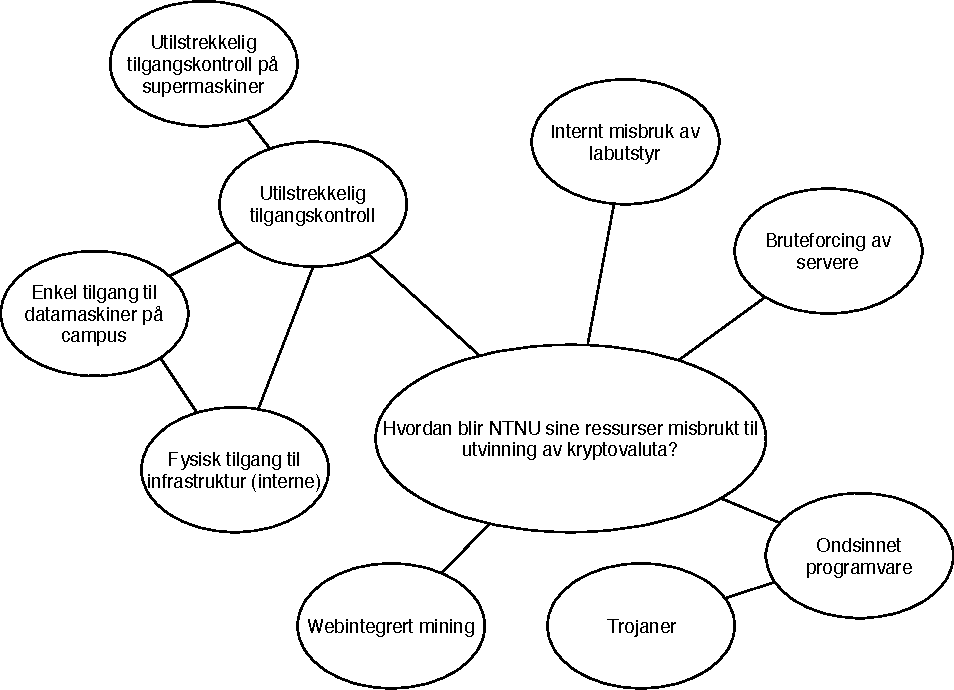
\includegraphics[scale=0.5]{case_3/bilder/idemyldring-hvordan.pdf}
    \caption[Idémyldring]{Resultater og gruppering av Hvordan}
     \label{fig:idemyldring-hvordan}
\end{figure}

\begin{figure}[H]
    \centering
    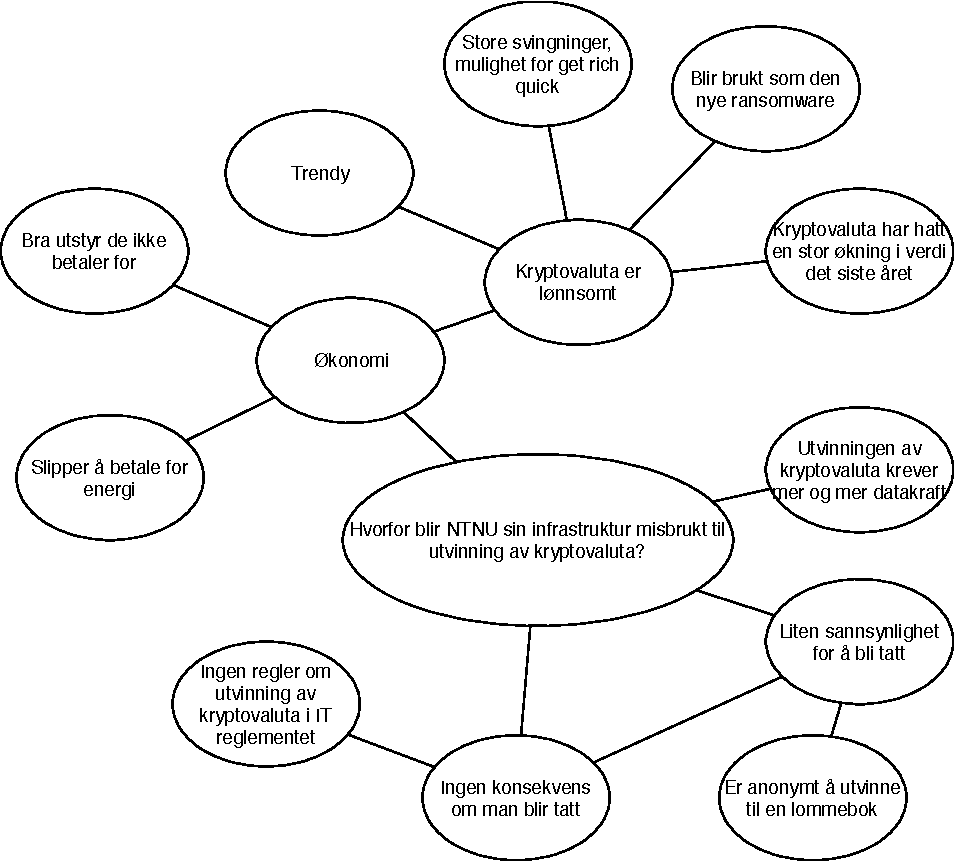
\includegraphics[scale=0.5]{case_3/bilder/idemyldring-hvorfor.pdf}
    \caption[Idémyldring]{Resultater og gruppering av Hvorfor}
    \label{fig:idemyldring-hvorfor}
\end{figure}

RESULTAT

\subsection{NGT}
Etter at hvert gruppemedlem hadde gitt ut sine 15 poeng satt vi igjen med 4 idéer som stakk seg ut med hvor mange poeng de fikk, disse er i fet skrift i tabell \ref{tab:NGT}. Disse fire årsakene er de vi kommer til å fokusere på i dette caset. De fire fokuspunktene kan deles etter de to problemstillingene ``hvordan og hvorfor''.

De to årsakene knyttet til ``hvorfor problemstillingen'' går ut på at det ikke er ulovlig med kryptoutvinning i henhold til gjeldende regelverk og faller derfor i en gråsone, der en ikke får noen represalier for å holde på med kryptoutvinning, annet enn å bli kastet av nettet. Konsekvensen kommer av at man ressurser utstyr til egen vinning.

De neste årsakene går ut på hvilke aktører som bruker universitetet sine ressurser til utvinning av kryptovaluta, og hvordan de bruker ressursene. Internt misbruk av labutstyr går ut på at studenter eller ansatte har tilgang til diverse labber og PCer som kan brukes til utvinning av kryptovaluta. Både ondsinnet programvare som utvinner kryptovaluta og webintegrerte utvinnere gjøres av eksterne aktører, disse pengene som tjenes her går som regel tilbake til diverse kriminelle nettverk. Det med utvinning av kryptovaluta har blitt mye mer utbredt som et alternativ til ransomware, der ransomware har blitt mindre lønnsomt i den siste tiden \cite{RW}.

\begin{table} [H]
    \begin{tabular}{ | m{2em} | m{30em} | m{3em} | }
        \hline
            \cellcolor{yellow}  & \cellcolor{yellow} \textbf{Årsak} & \cellcolor{yellow} Poeng \\
        \hline
           A& Bra utstyr de ikke betaler for & 5 \\
        \hline
          B & Bruteforce av servere & 0 \\
        \hline
          C & Enkel tilgang til datamaskiner på campus & 0 \\
        \hline
         \textbf{D} & \textbf{Ingen regler om utvinning av kryptovaluta i IT reglementet} & 11 \\
        \hline
          \textbf{E} & \textbf{Internt misbruk av labutstyr} & 8  \\
        \hline
          F & Kryptovaluta har hatt en stor økning i verdi det siste året & 0 \\
        \hline
         G & Liten sannsynlighet for å bli tatt & 2 \\
        \hline
         \textbf{H} & \textbf{Ondsinnet programvare som miner} &  16 \\
        \hline
         I & Slipper å betale for energi & 0 \\
        \hline
         J & Store svingninger, mulighet for “get rich quick" & 0 \\
        \hline
         K & Utilstrekkelig tilgangskontroll på supermaskiner & 0 \\
        \hline
         L & Utvinningen av kryptovaluta krever mer og mer datakraft & 4 \\
        \hline
         \textbf{M} & \textbf{Webintegret miner} & 14 \\
        \hline
    \end{tabular}
    \caption{Oversikt over prioritering av idéer ved hjelp av NGT}
    \label{tab:NGT}
\end{table}
%%%%%%%%%%%%%%%%%%%%%%%%%%%%%%%%%%%%%%%%%%%%%%%%%%%%%%%%%%%%%%%%%%%%%
\section{Datainnsamling}
\subsection{Spørreundersøkelse}
Før intervjuet fikk vi et utdrag av alarmer som SOCen får av de kjente signaturene som omhandler kryotoutvinning. Disse alarmene stammer fra ``utvinnere'' som folk har fått lagt inn på PCene sine, ``utvinnere'' i nettleser som er lagt inn i diverse nettsider eller trojanere. 

Vi hadde noen hypoteser når vi utformet intervjuspørsmålene, disse var:
\begin{itemize}
    \item Det er tekniske løsninger som kan brukes til å fikse store deler av problemet.
    \item Det er begrenset handlingsrom for hva som kan bli gjort mot interne som utvinner.
    \item Lite bevissthet rundt regelverket til NTNU angående bruk av universitetets ressurser.
    \item Utviklingen av utvinning følger kryptovalutaen sin verdi.
    \item Dataer blir kompromittert gjennom de vanlige formene, phishing og wateringholes.
\end{itemize}

\begin{table}[H]
    \centering
    \begin{tabular}{|m{30em}|} 
        \hline
             \cellcolor{yellow} Spørsmål  \\
        \hline
          Hva er de typiske angrepsvektorene?  \\
         \hline
         Tar det lang tid å oppdage trojanere i nettverket? \\ 
         \hline
         Hva gjør Seksjon for Digital Sikkerhet når de oppdager trojanere? \\
         \hline
         Hvordan fant dere ut om HPC clusterne blir misbrukt? \\
         \hline
         Hvordan fant dere ut at det var internt misbruk?\\
         \hline
         Har dere andre tiltak enn å stenge internett til de som miner? \\
         \hline
         hva er grunnen til at dere ikke har implementert noe slike tiltak? \\
         \hline
         Hva tror du er oppfatningen blant dine kollegaer er angående utvinning. Vet folk det er ulovlig eller har de ikke tenkt så mye over det og utvinner fordi det er en trend? \\
         \hline
         Hva er måten dere for du snakket tidligere om at dere så mange av de lommebøkene som ble brukt var fra mørke siden av nettet?  \\
         \hline
         Hvordan ser dere at de går til disse lommebøkene? \\
         \hline
          Hvordan skal dere implementere kryptoutvinning i neste IT-reglement? \\
          \hline
          Tenker folk over at det ikke er lov til å utvinne krypto i henhold til IT-reglementet? \\
          \hline
          Har dere noen tiltak på utvinning på nettsider? \\
          \hline
          Er det like stor økning nå som det var før jul? \\
          \hline
          Økningen er det gjort av de profesjonelle aktørene eller er det folk som setter frivillig opp utvinnere? \\
          \hline
          Dere hadde ikke sett noe tilfeller av brutforcede PCer og servere som ble installert kryptominere på, etter at de ble brutforcet?  \\
          \hline
          Er det noen regler på hva ansatte får lov til å legge på serverne? \\
          \hline
          Har dere noen tilfeller av PCer på datalabber der studenter har installert kryptoutvinning?
          \hline
    \end{tabular}
    \caption{Spørsmål til intervju case 3}
    \label{tab:spm-intervju}
\end{table}
Under intervjuet valgte vi å ta lydopptak, slik at vi lett kunne gå tilbake til svarene for å få det mest mulig nøyaktig til neste fase. Når intervjuet var ferdig transkriberte vi det.
%%%%%%%%%%%%%%%%%%%%%%%%%%%%%%%%%%%%%%%%%%%%%%%%%%%%%%%%%%%%%%%%%%%%%
\section{Dataanalyse}
\subsection{Affinitetsdiagram}
Affinitetsdiagram brukes til å analysere data som det ikke er mulig å nummerere, eksempelvis meninger eller ideer. Affinitetsdiagram grupperer data og finner de underliggende korrelasjoner og likhetstrekk i gruppen.

Analysen ble gjennomført med å ta transkripsjon av intervjuet og stykke den opp i fem hovedgrupper.     

\begin{figure}[H]
    \centering
    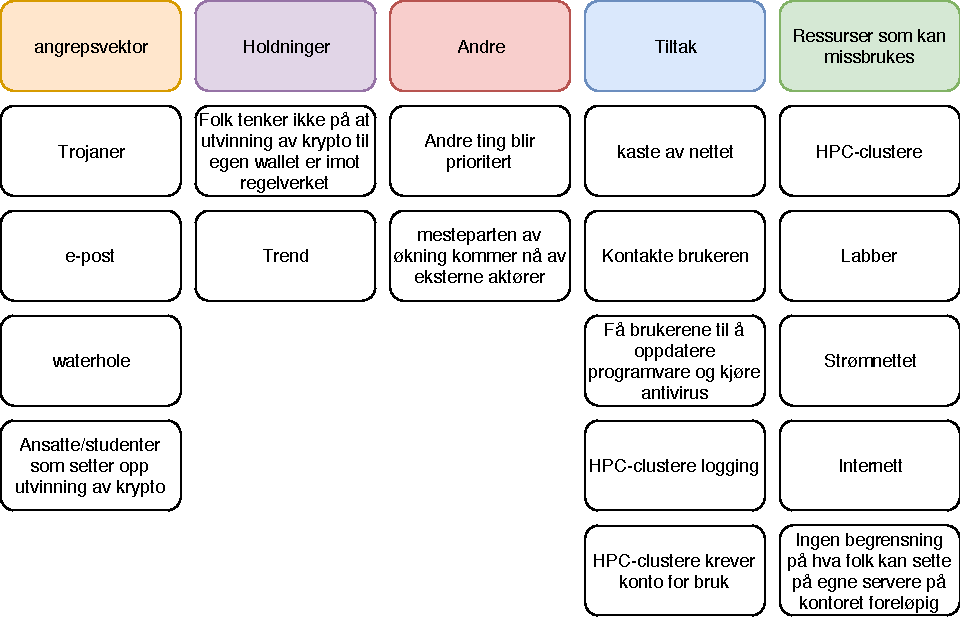
\includegraphics[scale=0.6]{case_3/bilder/AD.pdf}
    \label{fig:AD_miner}
    \caption{Hvordan fungerer utvinning av kryptovaluta ved NTNU?}
\end{figure}

Vi finner mulige årsaker og tiltak som er satt på plass, og forhåpentligvis er rotårsaken blant dem.

RESULTAT

%%%%%%%%%%%%%%%%%%%%%%%%%%%%%%%%%%%%%%%%%%%%%%%%%%%%%%%%%%%%%%%%%%%%%
\section{Rotårsaksidentifisering}
\subsection{5 whys}
Det ble fremhevet fem årsaker som skulle analyseres. Fire av disse kom fra fiskebeindiagrammet over, og en fra idémyldring. Tabellene under viser resultatene fra gjennomføringen. 

\begin{table} [H]
    \centering
    \begin{tabular}{ | m{5em} | m{30em} | }
        \hline
            \cellcolor{yellow} Årsak: & \cellcolor{yellow} Ansatte og studenter utvinner krypto med universitetet sine ressurser                \\
        \hline
            Why? & Lønnsomhet                                    \\
        \hline
            Why? & Har ingen utgifter                                            \\
        \hline
            Why? & Bruker strøm og infrastrukturen til skolen                \\
        \hline
            Why? & Det er en gråsone i regelverket           \\
        \hline
            Why? & Ikke spesifisert godt nok i IT-reglementet   \\
        \hline
    \end{tabular}
    \caption[5 Whys: Ansatte og studenter utvinner krypto med skolens]{5 Whys på ansatte og studenter utvinner krypto med skolens}
    \label{5Whys-interne}
\end{table}
Det å utvinne krypto på universitetet sine ressurser er alt fra å kjøre en kryptominer på en PC til å sette opp en mining rig. I 5 Whys over kom vi frem til at lønnsomhet er primærgrunnen til at de driver med kryptoutvinning, men årsaken til at ansatte og studenter utvinner på universitet er at det ikke er spesifisert godt nok i IT-reglementet.   


\begin{table} [H]
    \centering
    \begin{tabular}{ | m{5em} | m{30em} | }
        \hline
            \cellcolor{yellow} Årsak: & \cellcolor{yellow} Eksterne trusselaktører utvinner krypto med skolens ressurser              \\
        \hline
            Why? & Lønnsomhet                                   \\
        \hline
            Why? & Enkelt å spre minere                                           \\
        \hline
            Why? & Folk går inn på waterholes og trykker på phishingmail               \\
        \hline
            Why? & Brukeren var ikke oppmerksom nok på e-mailen eller siden de gikk på           \\
        \hline
            Why? & Brukere har ikke fått nok opplæring i hvordan dette unngås    \\
        \hline
    \end{tabular}
    \caption[5 Whys: Eksterne trusselaktører utvinner krypto med skolens ressurser]{5 Whys Eksterne trusselaktører utvinner krypto med skolens ressurser}
    \label{5Whys-eksterne}
\end{table}

Årsaken til at eksterne trusselaktører utvinner krypto med skolen sine ressurser er fordi det er en lønnsom affære som er koster lite å distribuere og som det er liten sannsynlighet for å bli tatt for. Med eksterne trusselaktører mener vi folk som utvinner på andre sine datamaskiner gjennom å få skadevare installert på disse.

\begin{table} [H]
    \centering
    \begin{tabular}{ | m{5em} | m{30em} | }
        \hline
            \cellcolor{yellow} Årsak: & \cellcolor{yellow} Utvinnere som implementert inn i nettsider              \\
        \hline
            Why? & God fortjeneste                                   \\
        \hline
            Why? & Fordi de når en stor menge folk som utvinner krypto for dem                                           \\
        \hline
            Why? & Mange har ikke en annonseblokkering som også stopper utvinnere på nett               \\
        \hline
            Why? & På grunn av lite eller ingen opplæring til denne typen programvare           \\
        \hline
            Why? & Ikke prioritert    \\
        \hline
            Why? & Fordi det ikke er nok folk/ressurser    \\
        \hline
    \end{tabular}
    \caption[5 Whys: Minere som er implementert inn i nettsider]{5 Whys på ansatte og studenter utvinner krypto med skolens}
    \label{5Whys-minere}
\end{table}

LEGG INN SISTE TEKST TIL 5 WHYS

\subsection{Feiltreanalyse}
Feiltreanalyse tar alle mulige årsaker i et diagram og identifiserer mulige linker. Analysen bygger på hva som ble gjort i 5 Whys.

Vi har kommet fram til fire hovedgrunner til at kryptoutvinning på NTNU forekommer. Rotårsaken er sammensatt av disse årsakene definert i figur \ref{fig:feil_tre_analyse}. I dette caset er problemet delt inn i to deler; de interne og de eksterne. Det er to forskjellige typer årsaker, der interne går mer på regelverk og eksterne er mer teknisk.          

I figur \ref{fig:feil_tre_analyse} representerer trekanter ``eller'', halvsirkelen representer ``og''. De røde boksene er de årsakene vi ikke kan gjøre noe med, de grønne kan det gjøres noe med.
 \begin{figure}[H]
    \centering
    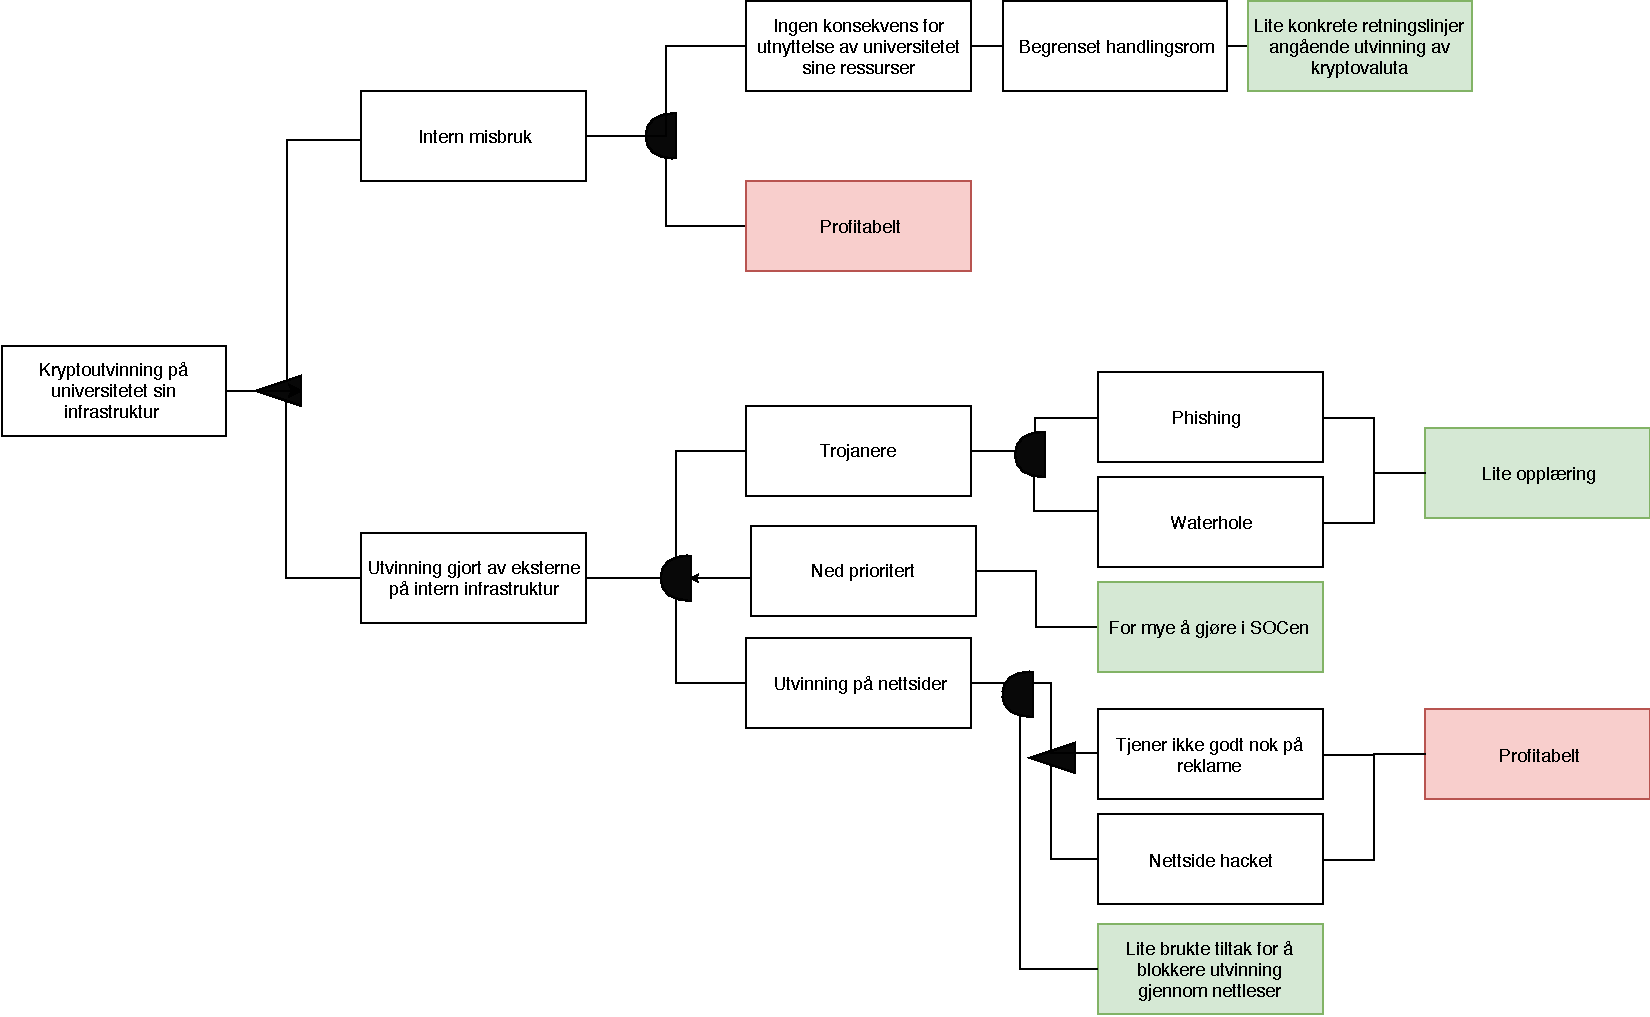
\includegraphics[scale=0.45]{case_3/bilder/feil_tre_analyse.pdf}
    \caption{Feiltreanalyse}
    \label{fig:feil_tre_analyse}
\end{figure}
%%%%%%%%%%%%%%%%%%%%%%%%%%%%%%%%%%%%%%%%%%%%%%%%%%%%%%%%%%%%%%%%%%%%%
\section{Rotårsakseliminering}
\subsection{SIT}
Alle komponenter som eksisterer i problemets naturlige omgivelser listes under:

\begin{itemize}
    \item IT-reglement
    \item Annonseblokker
    \item Internett
    \item SOCen
    \item Brannmur
    \item Servere og datamaskiner
    \item Datalabber
    \item HPC-cluster
    \item Bring your own device (BYOD)
    \item Strøm
\end{itemize}

Når komponentene er gjort rede for, vil de fem SIT prinsippene brukes sekvensielt på komponentene for å utvikle løsninger på problemene. Ikke alle SIT-prinsipper finner løsninger som er gjennomførbare for alle komponenter. I disse tilfellene vil det stå: ``Ikke gjennomførbart''. Resultatene fremheves under.

\paragraph{IT-reglement}
\begin{itemize}
    \item \textbf{Attributtavhengighet} Legge til et større fokus på utvinning av krypto.
    \item \textbf{Komponentkontroll} Gjennomføre en informasjonskampanje for å sette fokus på hva som er misbruk.
    \item \textbf{Erstatning} Ikke gjennomførbart.
    \item \textbf{Forkastning} Ikke gjennomførbart.
    \item \textbf{Oppdeling} Ikke gjennomførbart. 
\end{itemize}

\paragraph{Annonseblokker}
\begin{itemize}
    \item \textbf{Attributtavhengighet} Legge til blokkering av mining 
    \item \textbf{Komponentkontroll} Passe på at alle ansatte har annonseblokker installert som også stopper utvinning av krypto.
    \item \textbf{Erstatning} Ikke gjennomførtbart
    \item \textbf{Forkastning} Ikke gjennomførtbart
    \item \textbf{Oppdeling} Ikke gjennomførtbart.
\end{itemize}

\paragraph{Internett}
\begin{itemize}
    \item \textbf{Attributtavhengighet} Blokkere kryptoutvinning
    \item \textbf{Komponentkontroll} Automatisere at alle datamaskiner som utvinner krypto blir kastet av nettet.
    \item \textbf{Erstatning} Ikke gjennomførtbart.
    \item \textbf{Forkastning} Ikke gjennomførtbart.
    \item \textbf{Oppdeling} Ikke gjennomførtbart.
\end{itemize}


\paragraph{SOC}
\begin{itemize}
    \item \textbf{Attributtavhengighet} Øke antall ansatte.
    \item \textbf{Komponentkontroll} Økt prioritet til krypto.
    \item \textbf{Erstatning} Ikke gjennomførtbart.
    \item \textbf{Forkastning} Ikke gjennomførtbart.
    \item \textbf{Oppdeling} Gi forslag til implementering av tiltak til bachelorgrupper.
\end{itemize}

\paragraph{Servere og datamaskin}
\begin{itemize}
    \item \textbf{Attributtavhengighet} Strengere adgangskontroll.
    \item \textbf{Komponentkontroll} Ikke gjennomførtbart.
    \item \textbf{Erstatning} Ikke gjennomførtbart.
    \item \textbf{Forkastning} Ikke gjennomførtbart.
    \item \textbf{Oppdeling} Ikke gjennomførtbart.
\end{itemize}

\paragraph{Datalabber}
\begin{itemize}
    \item \textbf{Attributtavhengighet} Strengere adgangskontroll.
    \item \textbf{Komponentkontroll} Logging.
    \item \textbf{Erstatning} Svakere maskinvare på labbene.
    \item \textbf{Forkastning} Slutte å tilby labber, som kan brukes i sammenheng med krypto utvinning.
    \item \textbf{Oppdeling} Ikke gjennomførbart.
\end{itemize}

\paragraph{HPC-clustere}
\begin{itemize}
    \item \textbf{Attributtavhengighet} Øke tilgangskontrollen ytterligere.
    \item \textbf{Komponentkontroll} Ikke gjennomførbart.
    \item \textbf{Erstatning} Ikke gjennomførbart.
    \item \textbf{Forkastning} Ikke gjennomførbart.
    \item \textbf{Oppdeling} Ikke gjennomførbart.
\end{itemize}


\paragraph{Bring your own device (BYOD)}
\begin{itemize}
    \item \textbf{Attributtavhengighet} Ikke gjennomførbart.
    \item \textbf{Komponentkontroll} Kaste datamaskiner som ikke tilhører NTNU-personell av nettet slik at de manuelt må koble seg på igjen.
    \item \textbf{Erstatning} Ikke gjennomførbart.
    \item \textbf{Forkastning} Ikke gjennomførbart.
    \item \textbf{Oppdeling} Ikke gjennomførbart.
\end{itemize}

\paragraph{Strøm}
\begin{itemize}
    \item \textbf{Attributtavhengighet} Ikke gjennomførtbart
    \item \textbf{Komponentkontroll} Strømkvotering, overstiges kvoten må vedkommende betale for strømmen
    \item \textbf{Erstatning} Ikke gjennomførtbart
    \item \textbf{Forkastning} Ikke gjennomførtbart
    \item \textbf{Oppdeling} Ikke gjennomførtbart
\end{itemize}

Vi sorterer og beskriver de mest relevante idéer til videre utdyping:

\begin{description}
\item[Gjennomføre en informasjonskampanje om kommersielt misbruk av NTNU sin infrastruktur] Kampanjen skal få frem at det å bruke NTNU sine ressurser til kommersiell virksomhet bryter IT-reglementet, og at strøm inngår i NTNU sine ressurser.
\item[Legge til et større fokus på utvinning av krypto i IT-reglementet] Gi IT-reglement et større fokus på kryptoutvinning og klarere retningslinjer på hva som ikke er greit å gjøre.
\item[Legge til annonseblokker som stopper utvinning] Aktivere blokkering av utvinning-protokoll på annonseblokkere og passe på at alle har en annonseblokkeringstjeneste installert.
\item[Blokkere kryptoutvinning] Med dette mener vi å gjøre et eller flere tiltak som å blokkere DNS-forespørsel som omhandler kryptoutvinning.  
\item[Øke antall personell i SOC] SOC har mange oppgaver som er mer kritiske enn kryptoutvinning. Derfor foreslår vi å ansette flere, kanskje i kombinasjon med bacheloroppgaver.
\item[Strengere adgangskontroll] Begrenser tilgang til datalabber. 
\item[Logging] Øke bruk av logging  i datalabbene. 
\item[Kaste datamaskiner som ikke er kritisk infrastruktur av nettet] Ved midnatt blir alle datamaskiner eller servere som ikke er kritisk infrastruktur koblet av nettet og må manuelt koble seg på nettet igjen.
\end{description}

\subsection{Tiltaksplan}
Etter å ha brukt de fem SIT-prinsippene på hver komponent, og filtrert de, sitter vi igjen med et par idéer. I denne delen fremhever vi idéer i en tiltaksplan som vi anbefaler å implementere. 
Under beskrives de ulike tiltakene:

\begin{description}
    \item[Gjennomføre en informasjonskampanje om kommersielt misbruk av NTNU sin infrastruktur] Utvinning av kryptovaluta er en ny ting, hvor mange ikke er klar over hvordan universitetet sitt regelverk håndterer temaet. Vår anbefaling er å ha en kampanje der universitet informerer om hva som regnes som NTNU sine ressuser og hvordan disse ikke skal brukes til kommersiell virksomhet.
    \item[Legge til et større fokus på utvinning av krypto i IT-reglementet] Endre IT-reglementet slik at det blir tydelig at kryptoutvinning ikke er lovlig bruk av NTNU sine ressurser. 
    \item[Blokkere kryptoutvinning] Dette tiltaket går ut på å blokkere DNS-forespørsler tilknyttet kryptoutvinning. Slik at PCer som blir brukt i utvinning ikke kan hente nye oppgaver å løse. De velkjente DNSene blokkeres. Videre kan loggen bli benyttet for å legge nye domener inn i en svarteliste, eller justere de gamle DNSene.
    \item[Øke antall personell i SOC] SOCen kan ikke prioritere å stoppe utvinning av kryptovaluta. Derfor anbefaler vi å enten øke mengden personell i SOCen, eller gi utvikling av implementasjonsstrategi som en bachelor oppgave.
\end{description}

%%%%%%%%%%%%%%%%%%%%%%%%%%%%%%%%%%%%%%%%%%%%%%%%%%%%%%%%%%%%%%%%%%%%%
\section{Løsningsimplementering}
\subsection{Kraftfeltsanalyse} 
Kraftfeltsanalyse blir brukt å få vite hvilke styrker for og hvilke styrker mot implementering av tiltakene. Dette verktøyet gir en plan over hvilke tiltak som er lettest å gjennomføre.  

 Informasjonskampanjen og endringen i IT-reglementet bør gjøre i kombinasjon med hverandre. Der IT-reglementet får klartgjort at selv om kryptoutvinning ikke ulovlig i henhold til norsk lov, er det imot NTNU sitt IT-reglement så langt det ikke er søkt om. Når endringen er gjort, gjennomføres informasjonskampanjen.   
 Under, i tabell \ref{fig:kampanje} og \ref{fig:IT-reglement}, viser resultatene fra kraftfeltsanalyse på informasjonskampanje og endring i IT-reglementet.
 \begin{figure}[H]
    \hspace{2.2cm}
    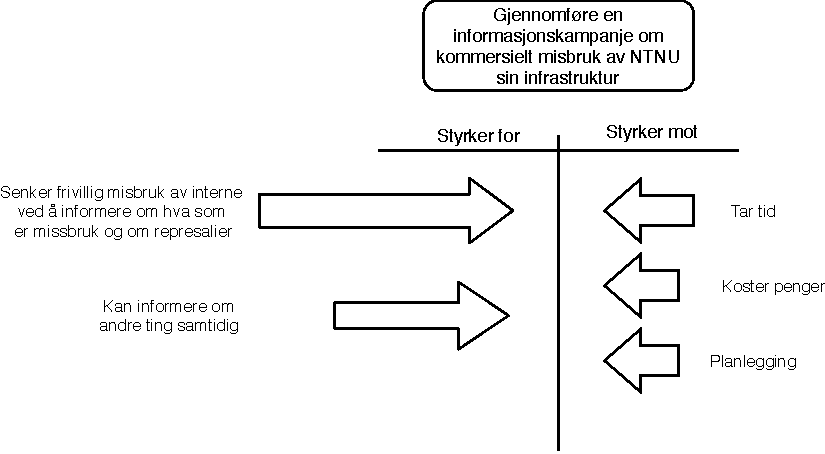
\includegraphics[scale=0.6]{case_3/bilder/Force-field1.pdf}
    \caption[Informasjonskampanje]{Oversikt over informasjonskampanjen }
    \label{fig:kampanje}
\end{figure}

 
 \begin{figure}[H]
    \hspace{2.6cm}
    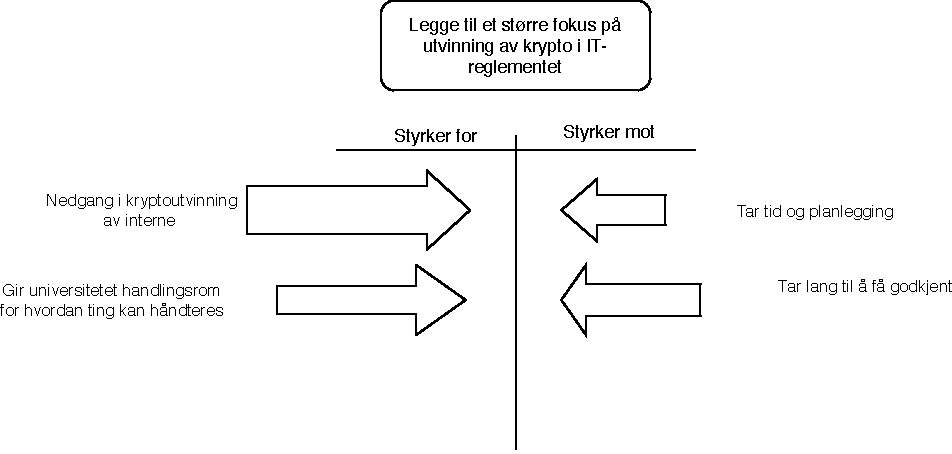
\includegraphics[scale=0.6]{case_3/bilder/Force-field2.pdf}
    \caption[Endre IT-reglementet]{Endring i IT-reglementet}
    \label{fig:IT-reglement}
\end{figure}

Fra dataanalysen kom fram til at selv om det finnes tekniske løsninger, har ikke SOCen hatt mulighet til å implementere DNS blokkering på bakgrunn av mangel på ressurser. Figur \ref{fig:Blokkering} og \ref{fig:Oke-antall} viser hva som skal til for å blokkere DNS og hva som må til for å øke ressursene til SOCen.    
 \begin{figure}[H]
    \centering
    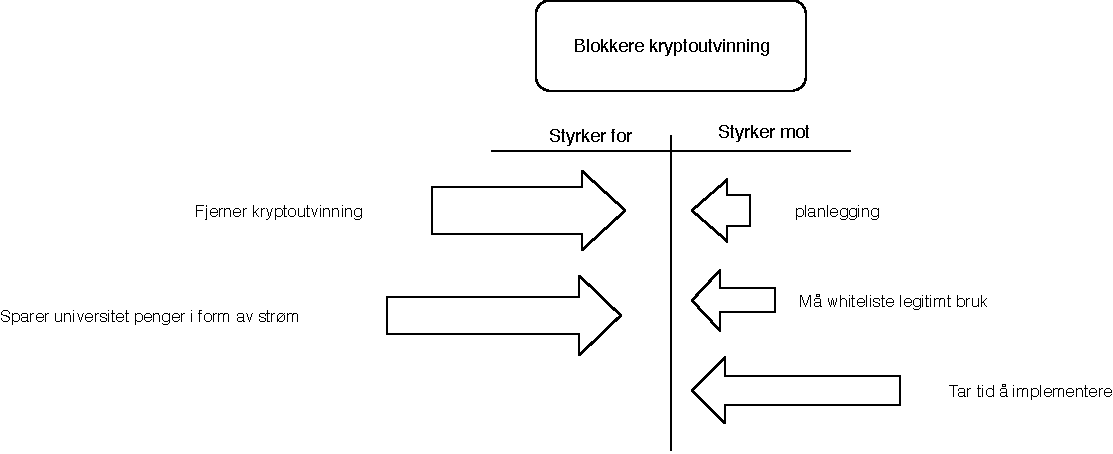
\includegraphics[scale=0.6]{case_3/bilder/Force-Field3.pdf}
    \caption[Blokkering]{Blokkering av DNS forespørsel}
    \label{fig:Blokkering}
\end{figure}

 \begin{figure}[H]
    \hspace{3.6cm}
    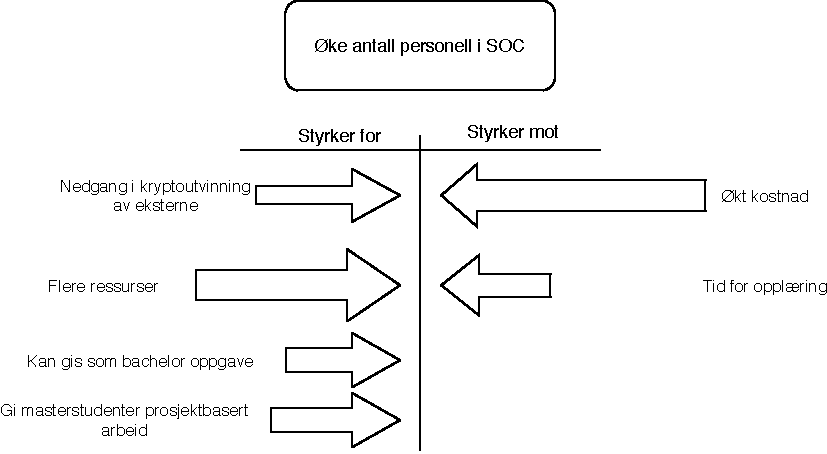
\includegraphics[scale=0.6]{case_3/bilder/Force-field4.pdf}
    \caption[Øke antall ansette i SOC]{Øke andel ansatte i SOC}
    \label{fig:Oke-antall}
\end{figure}

Figurene viser våres antakelser på hva som jobber for implementeringen og hva som jobber mot, samt estimater på styrken til antakelsene, der lengden indikerer antatt styrke. 
%%%%%%%%%%%%%%%%%%%%%%%%%%%%%%%%%%%%%%%%%%%%%%%%%%%%%%%%%%%%%%%%%%%%%
\section{Tidsbruk}
Tabell \ref{tab:tidsbruk_case3} under viser tidsbruken i enkeltfasene i dette caset. Dette inkluderer tid brukt til å dokumentere alt som har med de enkelte fasene å gjøre. 

% Table generated by Excel2LaTeX from sheet 'Ark1'
\begin{table}[H]
  \centering
  \caption{Tidsbruk de ulike fasene i case 3}
    \begin{tabular}{|lr|l|}
    \hline
    \multicolumn{3}{|c|}{\cellcolor{yellow}\textbf{Case 3}} \\
    \hline
    \multicolumn{1}{|l|}{\cellcolor{apricot}\textbf{Fase}} & \multicolumn{1}{l|}{\cellcolor{apricot}\textbf{Verktøy brukt}} & \cellcolor{apricot}\textbf{Timer totalt} \\
    \hline
    \multicolumn{1}{|l|}{Problemforståelse} & \multicolumn{1}{l|}{Ytelsesmatrise} & 16-20t \\
    \hline
    \multicolumn{1}{|l|}{Idémyldring} & \multicolumn{1}{l|}{Idémyldring og NGT} & 16-20t \\
    \hline
    \multicolumn{1}{|l|}{Datainnsamling} & \multicolumn{1}{l|}{Intervju} & 20-30t \\
    \hline
    \multicolumn{1}{|l|}{Datanalyse} & \multicolumn{1}{l|}{Affinitetsdiagram} & 15-20t \\
    \hline
    \multicolumn{1}{|l|}{Rotårsaksidentifisering} & \multicolumn{1}{l|}{5 whys og feil-tre diagram} & 25-30t \\
    \hline
    \multicolumn{1}{|l|}{Rotårsakseliminering} & \multicolumn{1}{l|}{SIT} & 15-20t \\
    \hline
    \multicolumn{1}{|l|}{Løsningsimplementering} & \multicolumn{1}{l|}{Kraftfeltsdiagram} & 10-15t \\
    \hline
    \multicolumn{2}{|l|}{\textbf{Sum}} & \textbf{117-155t} \\
    \hline
    \end{tabular}%
  \label{tab:tidsbruk_case3}%
\end{table}%
